% =====================================================================
\chapter{Modèles espace-état et filtre de Kalman}
\label{ch:8}
% =====================================================================

\section{Objectifs et organisation du chapitre}

\paragraph{Objectifs.} Les chapitres précédents ont supposé un ratio de couverture constant. Dans la réalité, la relation entre deux actifs dérive. Le filtre de Kalman estime en temps réel des quantités cachées qui évoluent (un ratio de couverture, la composante stationnaire d'un écart) à partir d'observations bruitées. À la fin du chapitre, vous saurez : (1) écrire un modèle espace-état ; (2) dériver les équations du filtre de Kalman à partir du conditionnement gaussien ; (3) l'appliquer à une régression à coefficients variables et à l'estimation de la cointégration partielle ; (4) régler ses paramètres sans tomber dans le piège de la vraisemblance ; (5) en tirer un signal de trading.

\paragraph{Code.} \texttt{code/ch08/ch08\_kalman.py}, expériences E1 à E5.

% =====================================================================
\section{Le modèle espace-état}
% =====================================================================

\begin{definition}
Un modèle espace-état linéaire gaussien comprend :
\begin{align*}
\text{équation d'état :}\quad & \xi_t = F\,\xi_{t-1} + w_t, & w_t\sim\N(0,Q),\\
\text{équation d'observation :}\quad & y_t = H_t\,\xi_t + v_t, & v_t\sim\N(0,R),
\end{align*}
où $\xi_t$ est l'état caché (non observé), $y_t$ l'observation, $F$ la matrice de transition, $H_t$ la matrice d'observation (qui peut dépendre du temps), et $w_t$, $v_t$ des bruits indépendants.
\end{definition}

\begin{intuition}
Vous suivez un bateau dans le brouillard. Vous savez à peu près comment il se déplace (équation d'état, avec une part d'imprévu), et de temps en temps un radar vous donne une position imprécise (équation d'observation). Le filtre de Kalman combine ces deux sources pour donner, à chaque instant, la meilleure estimation de la position et son incertitude. Il fait confiance au radar quand la prévision est incertaine, et à la prévision quand le radar est imprécis.
\end{intuition}

\paragraph{Exemples en arbitrage statistique.}
\begin{itemize}
\item \textbf{Ratio de couverture variable :} $\xi_t = (\alpha_t,\beta_t)^\top$ suit une marche aléatoire ($F = I$), et l'on observe $y_t = \alpha_t + \beta_tx_t + v_t$, donc $H_t = (1, x_t)$.
\item \textbf{Écart observé avec bruit} \citep{elliott2005} : l'état $\xi_t$ est un écart qui revient à la moyenne ($\xi_t = a + b\,\xi_{t-1} + w_t$, $|b|<1$) et l'on observe $y_t = \xi_t + v_t$, où $v_t$ représente le bruit de microstructure.
\item \textbf{Cointégration partielle} \citep{clegg2018} : $\xi_t = (M_t, R_t)^\top$, $F = \mathrm{diag}(\rho,1)$, et l'écart observé est $S_t = M_t + R_t$, donc $H = (1,1)$.
\end{itemize}

% =====================================================================
\section{Les équations du filtre}
% =====================================================================

\subsection{Un résultat de conditionnement gaussien}

\begin{lemma}\label{c8:lem:cond}
Si $(X, Y)$ est un vecteur gaussien de moyenne $(\mu_X,\mu_Y)$ et de covariances $\Sigma_{XX}$, $\Sigma_{XY}$, $\Sigma_{YY}$, alors la loi de $X$ sachant $Y = y$ est gaussienne de moyenne $\mu_X + \Sigma_{XY}\Sigma_{YY}^{-1}(y-\mu_Y)$ et de covariance $\Sigma_{XX} - \Sigma_{XY}\Sigma_{YY}^{-1}\Sigma_{YX}$.
\end{lemma}
\begin{proof}
Posons $Z = X - \Sigma_{XY}\Sigma_{YY}^{-1}Y$. Alors $\Cov(Z, Y) = \Sigma_{XY} - \Sigma_{XY}\Sigma_{YY}^{-1}\Sigma_{YY} = 0$. Pour un vecteur gaussien, covariance nulle signifie indépendance : $Z$ est indépendant de $Y$. Donc, sachant $Y = y$, $X = Z + \Sigma_{XY}\Sigma_{YY}^{-1}y$ a pour moyenne $\E[Z] + \Sigma_{XY}\Sigma_{YY}^{-1}y = \mu_X + \Sigma_{XY}\Sigma_{YY}^{-1}(y - \mu_Y)$ et pour covariance $\Var(Z) = \Sigma_{XX} - \Sigma_{XY}\Sigma_{YY}^{-1}\Sigma_{YX}$ (calcul direct avec la proposition~\ref{c1:prop:varspread} généralisée aux matrices).
\end{proof}

\subsection{Prédiction et mise à jour}

Supposons connue la loi de l'état sachant les observations jusqu'à $t-1$ : $\N(m_{t-1}, P_{t-1})$.

\begin{proposition}[Filtre de Kalman]\label{c8:prop:kalman}
\textbf{Prédiction :} $m_{t|t-1} = F m_{t-1}$, \quad $P_{t|t-1} = F P_{t-1}F^\top + Q$.

\textbf{Innovation :} $e_t = y_t - H_tm_{t|t-1}$, de variance $F_t = H_tP_{t|t-1}H_t^\top + R$.

\textbf{Mise à jour :} $K_t = P_{t|t-1}H_t^\top F_t^{-1}$, \quad $m_t = m_{t|t-1} + K_te_t$, \quad $P_t = P_{t|t-1} - K_tH_tP_{t|t-1}$.
\end{proposition}
\begin{proof}
La prédiction découle de l'équation d'état : $\E[F\xi_{t-1} + w_t] = Fm_{t-1}$ et $\Var(F\xi_{t-1} + w_t) = FP_{t-1}F^\top + Q$, car $w_t$ est indépendant du passé. Sachant le passé, le couple $(\xi_t, y_t)$ est gaussien, avec $\E[y_t] = H_tm_{t|t-1}$, $\Var(y_t) = H_tP_{t|t-1}H_t^\top + R = F_t$ et $\Cov(\xi_t, y_t) = P_{t|t-1}H_t^\top$. Le lemme~\ref{c8:lem:cond} avec $X = \xi_t$, $Y = y_t$ donne exactement la mise à jour.
\end{proof}

\paragraph{Lecture dans le cas scalaire.} Avec un état et une observation de dimension 1 et $H = 1$, le gain vaut $K = P/(P+R)$. Si la prévision est très incertaine ($P\gg R$), $K\approx1$ et l'on suit l'observation ; si l'observation est très bruitée ($R\gg P$), $K\approx0$ et l'on garde la prévision. La nouvelle estimation est une moyenne pondérée de la prévision et de l'observation, et sa variance $P(1-K) = PR/(P+R)$ est plus petite que chacune des deux.

\subsection{Vraisemblance}

Les innovations $e_t$ sont indépendantes et de loi $\N(0, F_t)$ sous le modèle. La log-vraisemblance s'écrit donc simplement (décomposition par erreurs de prévision) :
\[
\ell = -\frac12\sum_t\Big(\ln(2\pi F_t) + \frac{e_t^2}{F_t}\Big).
\]
On estime les paramètres inconnus ($Q$, $R$, $\rho$\dots) en maximisant $\ell$, comme au chapitre~2.

% =====================================================================
\section{Ratio de couverture variable}
% =====================================================================

\subsection{Le modèle}

On pose $\xi_t = (\alpha_t, \beta_t)^\top$, $F = I$, $Q = \frac{\delta}{1-\delta}I$ et $H_t = (1, x_t)$, suivant la paramétrisation popularisée par \citet{chan2013} : $\delta$ règle la vitesse à laquelle les coefficients peuvent changer. Avec $\delta\to0$, les coefficients sont constants et le filtre converge vers les MCO récursifs ; avec $\delta$ grand, ils suivent chaque mouvement.

\begin{codebox}[ — E1 et E2, suivi d'un ratio qui dérive]
\textbf{Protocole :} prix simulés, $y_t = 5 + \beta_tx_t + s_t$ avec $\beta_t$ marche aléatoire (pas d'écart-type $0{,}003$) et $s_t$ AR(1) ($\varphi = 0{,}9$) ; 1\,500 jours. \textbf{Erreur quadratique moyenne sur $\beta_t$} (après 250 jours) : Kalman $0{,}017$ avec $\delta = 10^{-7}$ ; $0{,}031$ avec $10^{-6}$ ; $0{,}061$ avec $10^{-5}$ ; $0{,}091$ avec $10^{-4}$. MCO glissants : $0{,}113$ (60 jours), $0{,}039$ (250 jours) ; MCO statique sur la formation : $0{,}048$. \textbf{Log-vraisemblance} : maximale pour $\delta = 10^{-5}$ ($-1\,370$), contre $-1\,928$ pour $\delta = 10^{-7}$.
\end{codebox}

\begin{figure}[h]
\centering
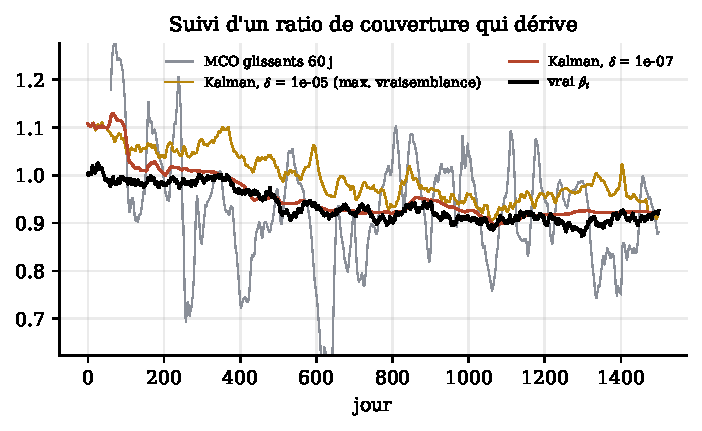
\includegraphics[width=0.75\textwidth]{ch08/kalman_beta.pdf}
\caption{Vrai ratio de couverture (noir), estimations par MCO glissants sur 60 jours, et par filtre de Kalman avec deux réglages. Le réglage qui maximise la vraisemblance (or) suit trop nerveusement ; le réglage lent (rouge) suit la vraie dérive.}
\label{c8:fig:beta}
\end{figure}

\subsection{Le piège de la vraisemblance}

Le réglage qui maximise la vraisemblance n'est pas celui qui suit le mieux $\beta_t$. La raison est importante : dans notre modèle, l'écart $s_t$ est autocorrélé, alors que le filtre suppose un bruit d'observation $v_t$ indépendant. Pour mieux prédire $y_t$, le filtre a intérêt à faire bouger $\alpha_t$ et $\beta_t$ pour absorber la partie prévisible de l'écart. Il gagne en vraisemblance\dots{} en \og mangeant\fg{} l'écart que l'on veut justement trader.

\begin{pitfall}
Un filtre de Kalman trop réactif fait disparaître le signal de retour à la moyenne dans l'état. Le critère de réglage doit correspondre à l'usage : pour un ratio de couverture, choisir $\delta$ petit (ou estimer $\delta$ sur un modèle qui inclut explicitement l'écart comme état AR(1), à la manière d'\citet{elliott2005}) et vérifier hors échantillon le P\&L de la stratégie, pas seulement la vraisemblance.
\end{pitfall}

\subsection{Un signal de trading}

L'innovation $e_t$ est l'écart entre le prix observé de $y$ et sa valeur prédite par la relation estimée : c'est un \emph{spread} à ratio variable, et $\sqrt{F_t}$ son écart-type prédit. Une règle simple : vendre l'écart quand $e_t > \sqrt{F_t}$, l'acheter quand $e_t < -\sqrt{F_t}$, fermer quand $e_t$ change de signe ; le P\&L utilise le ratio de la veille, pour ne pas anticiper.

\begin{codebox}[ — E3, Kalman contre ratio statique]
\textbf{Protocole :} 100 paires simulées avec $\beta_t$ qui dérive, formation de 250 jours, trading de 750 jours, coûts de 5 pb par jambe. \textbf{Résultats} (rendement annuel sur le notionnel brut) : Kalman ($\delta = 10^{-6}$) $6{,}5\,\%$ en moyenne (écart-type $4{,}2\,\%$, 99\,\% de paires gagnantes) ; ratio statique et \emph{z-score} à 2 : $1{,}7\,\%$ (écart-type $2{,}4\,\%$, 72\,\% de paires gagnantes).
\end{codebox}

Quand le ratio dérive réellement, le filtre maintient un écart stationnaire là où le ratio statique laisse l'écart dériver. Quand le ratio est stable (chapitre~7, E4), un filtre lent se comporte comme les MCO et ne coûte presque rien : c'est une assurance peu chère.

% =====================================================================
\section{Estimer la cointégration partielle}
% =====================================================================

Avec l'état $(M_t, R_t)$, $F = \mathrm{diag}(\rho,1)$, $Q = \mathrm{diag}(\sigma_M^2,\sigma_R^2)$, $H = (1,1)$ et un bruit d'observation négligeable, le filtre décompose l'écart observé en une partie qui revient à la moyenne et une partie qui dérive. On estime $(\rho,\sigma_M,\sigma_R)$ par maximum de vraisemblance.

\begin{codebox}[ — E5, cointégration partielle]
\textbf{Protocole :} vrais paramètres $\rho = 0{,}8$, $\sigma_M = 1$, $\sigma_R = 0{,}4$ ($R^2_{MR} = 0{,}874$), 25 écarts de 1\,000 points. \textbf{Résultats} (médianes) : $\hat\rho = 0{,}801$, $\hat\sigma_M = 1{,}005$, $\hat\sigma_R = 0{,}379$, $\hat R^2_{MR} = 0{,}880$ ; intervalle 5–95\,\% de $\hat\rho$ : $[0{,}73\,;\,0{,}84]$. Rappel : sur ce type d'écart, le test ADF du chapitre~4 échouait souvent à détecter quoi que ce soit.
\end{codebox}

En trading, on utilise l'estimation filtrée $\hat M_t$ (et non l'écart brut) pour le signal : on parie sur le retour de la composante stationnaire, pas sur celui de la marche aléatoire.

% =====================================================================
\section{Études de cas réelles}
% =====================================================================

\begin{codebox}[ — E4, ratio de Kalman sur données réelles ($\log$-prix, $\delta = 10^{-5}$)]
\textbf{KO sur PEP :} $\hat\beta_t$ passe de $0{,}76$ (après 30 séances) à $0{,}52$ au milieu de l'échantillon et finit à $0{,}58$. \textbf{GLD sur GLDM :} $\hat\beta_t$ part de $1{,}20$ et converge vers $1{,}02$.
\end{codebox}

\begin{figure}[h]
\centering
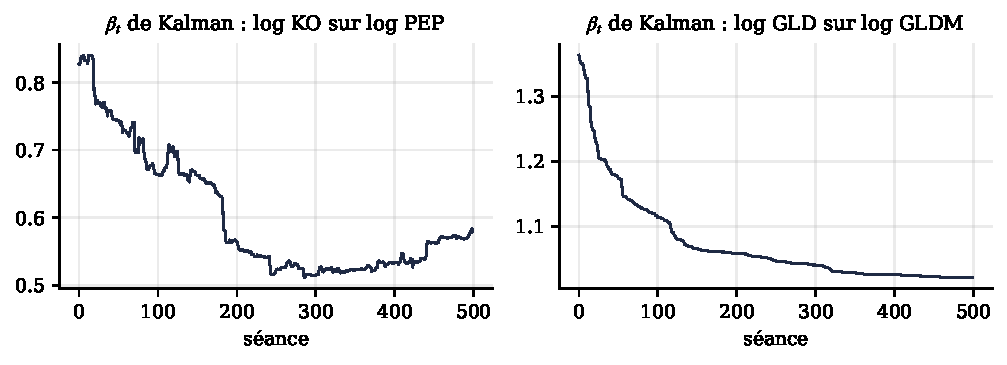
\includegraphics[width=0.95\textwidth]{ch08/kalman_reel.pdf}
\caption{Ratio de couverture estimé par filtre de Kalman sur les log-prix réels.}
\label{c8:fig:reel}
\end{figure}

\paragraph{Lecture.} Pour GLD/GLDM, le vrai ratio en log vaut 1 ; le départ à $1{,}20$ vient de l'initialisation et d'une difficulté d'identification : quand $\log x_t$ varie peu autour d'un niveau élevé (ici $\log 80\approx4{,}4$), l'ordonnée $\alpha_t$ et la pente $\beta_t$ peuvent se compenser. Pour KO/PEP, le ratio local est positif (les deux titres bougent ensemble au jour le jour) alors que la régression statique sur deux ans donnait un ratio négatif (les niveaux ont divergé) : le filtre mesure une relation de court terme, ce qui ne garantit pas un écart stationnaire.

\begin{pitfall}
Avec des log-prix, centrez la variable explicative (régressez sur $\log x_t - \overline{\log x}$) ou fixez l'ordonnée pour éviter la compensation entre $\alpha_t$ et $\beta_t$. Et ne jugez jamais un filtre sur ses premières dizaines d'observations, qui reflètent surtout l'initialisation.
\end{pitfall}

% =====================================================================
\section{Ce que la théorie apporte, et ses limites}
% =====================================================================

\paragraph{Apports.} Un estimateur récursif, optimal sous hypothèses gaussiennes, qui donne à chaque instant une estimation et son incertitude ; un cadre unique pour les ratios variables, les écarts bruités et la cointégration partielle ; une vraisemblance qui permet d'estimer les paramètres.

\paragraph{Limites.} Optimalité seulement si le modèle est juste (linéaire, gaussien, bruits indépendants) ; sensibilité au réglage de $Q$ et $R$, avec le piège de la vraisemblance quand le modèle est mal spécifié ; initialisation et identification délicates ; un ratio qui s'adapte peut aussi \og suivre\fg{} une rupture au lieu de la signaler.

% =====================================================================
\section{Fiche à recopier au tableau blanc}
% =====================================================================

\begin{whiteboard}
\begin{itemize}[leftmargin=1.2em]
\item \textbf{Modèle :} $\xi_t = F\xi_{t-1} + w_t$ ($Q$) ; $y_t = H_t\xi_t + v_t$ ($R$).
\item \textbf{Conditionnement :} $\E[X|y] = \mu_X + \Sigma_{XY}\Sigma_{YY}^{-1}(y-\mu_Y)$ ; $\Var = \Sigma_{XX} - \Sigma_{XY}\Sigma_{YY}^{-1}\Sigma_{YX}$.
\item \textbf{Prédiction :} $m^- = Fm$, $P^- = FPF^\top + Q$.
\item \textbf{Innovation :} $e = y - Hm^-$, $F_t = HP^-H^\top + R$.
\item \textbf{Mise à jour :} $K = P^-H^\top F_t^{-1}$, $m = m^- + Ke$, $P = P^- - KHP^-$.
\item \textbf{Scalaire :} $K = P/(P+R)$.
\item \textbf{Vraisemblance :} $\ell = -\frac12\sum(\ln 2\pi F_t + e_t^2/F_t)$.
\item \textbf{Ratio variable :} $\xi = (\alpha,\beta)$, $F = I$, $Q = \frac\delta{1-\delta}I$, $H_t = (1,x_t)$ ; signal $e_t/\sqrt{F_t}$.
\end{itemize}
\end{whiteboard}

% =====================================================================
\section{Exercices}
% =====================================================================

\begin{exercise}
Dans le cas scalaire avec $F = 1$, $H = 1$, montrez que la variance $P_t$ converge vers une valeur stationnaire $P^\ast$ solution de $P^\ast = (P^\ast+Q)R/(P^\ast+Q+R)$. Calculez $P^\ast$ et le gain stationnaire pour $Q = 1$, $R = 4$.
\end{exercise}

\begin{exercise}
Montrez que si $Q = 0$ et $F = I$, le filtre de Kalman de la régression à coefficients variables donne, à chaque date, l'estimateur MCO calculé sur toutes les observations passées (avec un a priori diffus).
\end{exercise}

\begin{exercise}
Expliquez pourquoi, dans le modèle d'\citet{elliott2005} où l'écart est un état AR(1) observé avec bruit, la variance du bruit d'observation réduit l'autocorrélation apparente de l'écart observé.
\end{exercise}

\begin{exercise}[à coder]
Réécrivez E1 avec la variable explicative centrée et comparez les trajectoires de $\hat\beta_t$ pour GLD/GLDM. La convergence initiale est-elle plus rapide ?
\end{exercise}

\begin{exercise}[à coder]
Ajoutez au modèle de ratio variable un troisième état, l'écart AR(1), et estimez $\delta$, $\varphi$ et la variance de l'écart par maximum de vraisemblance. Le $\delta$ estimé est-il proche du réglage qui suit le mieux $\beta_t$ ?
\end{exercise}

% =====================================================================
\section{Pour aller plus loin}
% =====================================================================

\begin{toread}
\begin{itemize}[leftmargin=1.2em]
\item \citet{hamilton1994}, chapitre~13 (\og The Kalman Filter\fg) : dérivation complète, vraisemblance et lissage.
\item \citet{elliott2005} : le modèle d'écart caché et son estimation.
\item \citet{chan2013}, chapitre~3 : le filtre de Kalman appliqué au ratio de couverture d'une paire d'ETF, avec code.
\item \citet{clegg2018} : estimation de la cointégration partielle par filtre de Kalman.
\end{itemize}
\end{toread}

\section{Scripts du chapitre}
\noindent\texttt{code/ch08/ch08\_kalman.py} : E1–E2 (figure~\ref{c8:fig:beta}), E3, E4 (figure~\ref{c8:fig:reel}), E5.
